\documentclass[12pt]{b-thesis}
\usepackage{ascmac,amsmath,amssymb,amsthm}
\usepackage[dvipdfmx]{graphicx}
\usepackage{multirow}
\usepackage{float}
\usepackage{slashbox}
\usepackage{comment}
\usepackage[tableposition=top]{caption}
%% pdf のしおり を作る
\usepackage[dvipdfmx,%
bookmarks=true,bookmarksnumbered=true,bookmarkstype=toc,%
colorlinks=true,% 
%colorlinks=false,%
linkcolor=black,%
citecolor=black,%
filecolor=black,%
%pagecolor=black,%
urlcolor=black%
]{hyperref}
%% pdf の しおり をEUCから unicode へ変換
\AtBeginDvi{\special{pdf:tounicode EUC-UCS2}}
\begin{document}
%%%%     Title    %%%%%
\typeout{Titlepage}
\title{Lightweight Network Function Chaining Mechanism \\ in Linux Kernel}
\teacher{寺岡 文男 教授}
\subteacher{金子}
\course{情報工学}
\id{61419670}
\author{吉用 ハンナ}
\maketitle

%%%%   Abstract   %%%%%
\typeout{Abstracts} 
\jabst{
\large
	Traditionally telecommunication networks have managed proprietary hardware to provide network functions (NF) such as P-GW and S-GW. To add flexibility of deploying NF, Network Function Virtualization (NFV) has emerged. NFV leverages virtualization technologies: VM-based  or container-based virtualization. However virtualization involves overhead in terms of memory copy in forwarding data and resource consumption to make instances. 
	
	To reduce the above overheads, this thesis propose lightweight NF chaining mechanism in Linux. The overall idea is that simple NFs are  chained in the kernel and only complicated NFs are placed in the user space, thus minimizing the cost of virtualization. NFs in kernel consist of kernel modules. A NF chain is a list that has nodes containing functions in the kernel. NFs can directly access the packet with pointer because they are all in the same memory region. 
	
	Chaining mechanism is implemented in the network stack before the routing subsystem. Only specified flows are processed by their corresponding NF chains. In addition to chaining mechanism, DoS attack detection/prevention and destination network address translation (DNAT), are implemented. 
	
	By using the implemented modules above, I confirmed that the NF chaining mechanism operates correctly. To measure the performance of NF chaining, experiment of processing two flows at 1Gbps is conducted. Memory usage increased only by a few tens of kilobytes compared to when idle and CPU utilization remained nearly 0\%. And the average throughput of received flows only fell by a few Mbytes compared to the throughput of destination prefix based forwarding on generic OS. These results indicates that the proposing NF chaining mechanism is lightweight in terms of resource consumption and yields line-rate throughput in a few Gbps traffic. 	
} 
\makejabstract 

\clearpage

%%%%     目次     %%%%%
\typeout{Indexes}

\setcounter{page}{1}
\pagenumbering{roman}

\tableofcontents
\thispagestyle{plain}

\listoffigures   %%% 図目次
\listoftables    %%% 表目次

\clearpage
%----------------------------------------------------------------------
%%%%     Body    %%%%%
\typeout{Main part}
%\setlength{\baselineskip}{16pt}

\pagestyle{headings}
\setcounter{page}{1}
\pagenumbering{arabic}

\clearpage

\chapter{序論}
\label{chap:intro}
\section{Network Function Chaining Infrastructure based on Virtualization Technologies} 
\subsection{Network Function Virtualization}
Traditionally carrier network has provided network functions (NF) like P-GW and S-GW on proprietary, dedicated hardware. However these hardware-based NFs have been being replaced by software, because of its high installation cost and relatively short lifetime. Furthermore flexible deployment of NF is required for the upcoming 5G wireless and Internet of Things (IoT). Since the software-based NFs are decoupled from the platform hardware, it is easy to newly deploy NF or withhold NF. 

Implementation of NF in software is realized by virtualization technology. This is called Network Function Virtualization (NFV). Virtualization technology is categorized into virtual machine (VM)-based and container-based technology. The former is full virtualization which creates virtual instances of hardware like CPU, RAM and network interface for every VM. Therefore a VM runs on a full copy on an operation system (OS) and virtual emulation of all needed hardware. A NF that runs as a VM is for these reasons resource consuming. The latter uses container-based technology represented by Docker\cite{Docker}. Container is a loosely isolated environment which runs on the kernel of host node. Isolation is done using five namespaces: process, network, mount, hostname, and shared memory. In contrast to VM, containers are light-weighted because each of them does not require virtualized resources.  

There are two main advantages in the virtualization technology. The first advantage of using them is the portability of NFs. Any NF that runs on a VM or container instance can operate on any host that supports the virtualization technologies. In case of KVM-based\cite{KVM} VM, a configuration file written by XML file and image file (raw or qcow format) and in case of Docker-based container, with Dockerfile (configuration file) and Docker image (disk image file) the same instance can be build. The second advantage is that the isolation is provided between instances (VMs or Containers). This enables the CPU and memory resources to be allocated to the instance as required. And the instance cannot take up more resources than allocated. 

Because of those advantages, VM and container are used very commonly in NFV. A host can have multiple NFs (VMs or containers), and the traffic between NFs are exchangeable with software switches. Combined with software-defined network (SDN), traffic can be managed to go through specific NFs in other hosts. Either by chaining NFs in a single host or between several hosts, a network service is created. This thesis proposes a novel NF chaining mechanism inside of the kernel in a single host. 

\subsection{Packet Forwarding in Virtualized Nodes}
In this chapter the detail of packet forwarding between the NIC of host and virtualized nodes like VM or container is explained. 

In case of VM-based NFV, packet forwarding consists of three architectures, packet I/O, virtual network I/O and virtual switch. 
\begin{enumerate}
	\item Packet I/O: 
	 Packet I/O is the part where packets pass through between physical NIC and user space. The default of Linux is NAPI (New API)\cite{NAPI}, but since the network stack of NAPI is considered redundant, there are acceleration technology like Intel DPDK\cite{DPDK}, XDP (eXpress Data Path)\cite{XDP} and Netmap\cite{Netmap} to bypass network stack. DPDK provides libraries that enables user space process to directly access physical NIC's packet buffer. XDP and Netmap use memory mapping between NIC's packet buffer and user space's shared memory region, to give user space application direct access to packets. 
	\item Virtual network I/O: 
	Virtual network I/O mechanism is used for networking VMs and the underlying hypervisor. In KVM, each host (VM) has virtio\cite{virtio} buffer in the guest host where outgoing or incoming packets are stored. For the connection of the virtio buffer and the socket buffer in the hypervisor host, TAP interface is used. TAP interface is a software device with two endpoints: one is a NIC and the other one is a file descriptor (fd). KVM process in the hypervisor sends traffic to the fd endpoint of the TAP device. The traffic then arrives at the NIC endpoint which can be connected to other NIC or TAP interface using a virtual switch. Finally the packets are written to the virtio buffer of the host. The reversed path (traffic from host to hypervisor) is vice versa. Since writing to the virtio buffer is done by KVM process in user space, it involves system calls every time. To reduce the overhead by system call, vhost-net\cite{vhost-net} is available in KVM. With vhost-net enabled, kernel thread directly writes to the virtio buffer from TAP device, in stead of KVM process in the user space. 
	\item Virtual switch: 
	Virtual switch is used to forward traffic to the right port as mentioned above. Open vSwitch (OVS)\cite{OVS}, which supports OpenFlow\cite{OpenFlow} is representative among others. OVS uses flow table which has match part and action part. Match part is set of rules to filter packet and can distinguish not only 5 tuples, but also VLAN tags or incoming port, etc. Action part can be drop, modify or transmit packet. When OVS works with virtual network I/O to realize NF chaining, the action should be transfer to specific Layer-2 (L2) address port. 
\end{enumerate}

In case of container-based NFV, packet forwarding is organized as follows. 
By default, Docker uses local private virtual network in the host. It creates virtual bridge and allocates subnet from one of the private address blocks. Each container gets allocated virtual ethernet device which is attached to the interface. In this way, containers in the same subnet can communicate, if they are on the same host. 

Kubernetes project\cite{Kubernetes} makes communication between containers on different hosts possible. Instead of allocating private IP address, Kubernetes gives each pod (a group of containers) a global IP address, allowing NAT-less, flat address space. Either in the normal networking or Kubernetes's networking, network stack in the host is used to reach containers. 

\section{Overhead of NFCI based on Virtualization Technologies}
\subsection{Memory copy}
The recently dominating trend in NFV is to use VM or Docker container to create Virtualized Network Function (VNF). However both of the technologies are not originally built in purpose of achieving high performance in heavy load network. 
Various kinds of efforts have been made to reduce the overhead of packet forwarding as mentioned in Sec. 1.1.3. For example, Netmap maps packet buffer into a memory region which user space process can directly access (zero-copy). But for the interaction with VM, software switch VALE\cite{VALE} which is supported on Netmap copies packets from the memory region to the guest's virtio buffer. Similary in case of DPDK + OVS, memory copy is needed to deliver traffic to VM. I believe that unnecessary memory copy should be avoided not to make possible bottleneck of data forwarding in NF chaining. 

Figure \ref{fig: kvm+ovs} shows the path of the traffic in a VM-based NFV instance with KVM as virtual network I/O and OVS as virtual switch. With NAPI, traffic go through network stack (packet I/O) of the host, bridging by OVS, get input to virtio buffer of the guest and passed again through network stack in the guest. Even when bypassing packet I/O with DPDK or Netmap, traffic has to proceed unnecessary layers in order to be processed in a NF. 

Figure \ref{fig: docker} shows the path of the traffic when containers are used to make NFs and Docker Engine such as Kubernetes supports networking between them. Since container uses host's OS, traffic does not need to pass network stack once more inside the container, as in the case of VM-based node. But the path all the way up from NIC to user space and forwarding data in Docker Engine is yet not optimized for a truly high performance NFV node. 

\subsection{Resource Consumption}
In case of VM-based NFV, a NF consists of one or multiple VMs. To launch a VM, virtual instances such as CPU, memory and network I/O must be created. Since virtual instances are allocated for each of the VM, when managing several VMs it consumes lot of hardware resources. 

\begin{figure}[t]
	\begin{minipage}{0.5\hsize}
		\begin{center}
			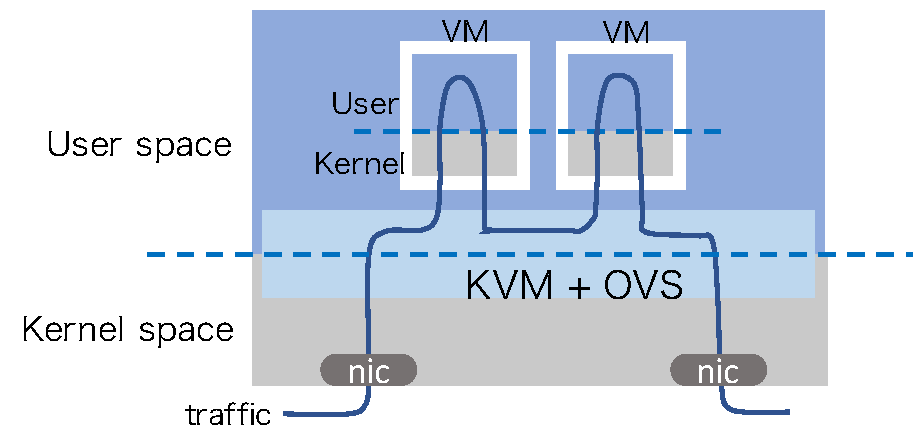
\includegraphics[width=85mm]{pics/KVM+OVS.pdf}
		\end{center}
		\caption{Traffic in VM-based NFV node}
		\label{fig: kvm+ovs}
	\end{minipage}	
	\begin{minipage}{0.5\hsize}
		\begin{center}
			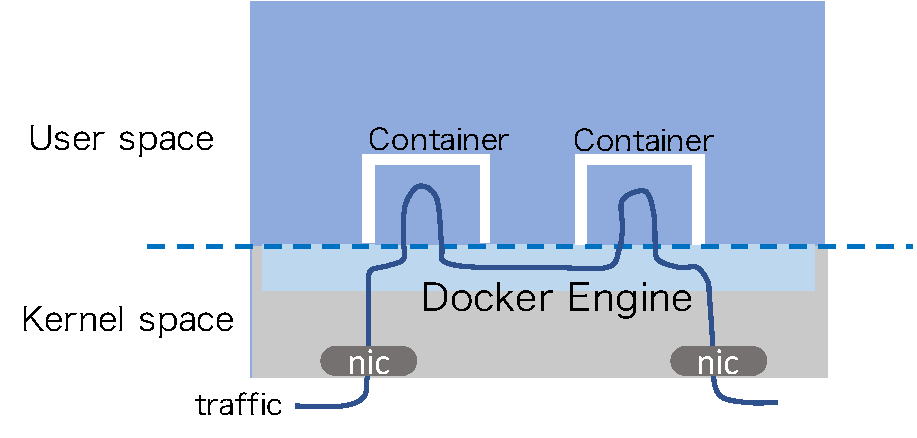
\includegraphics[width=85mm]{pics/Docker.pdf}
		\end{center}
		\caption{Traffic in Container-based NFV node}
		\label{fig: docker}
	\end{minipage}	
\end{figure}

\begin{figure*}
	\centering
	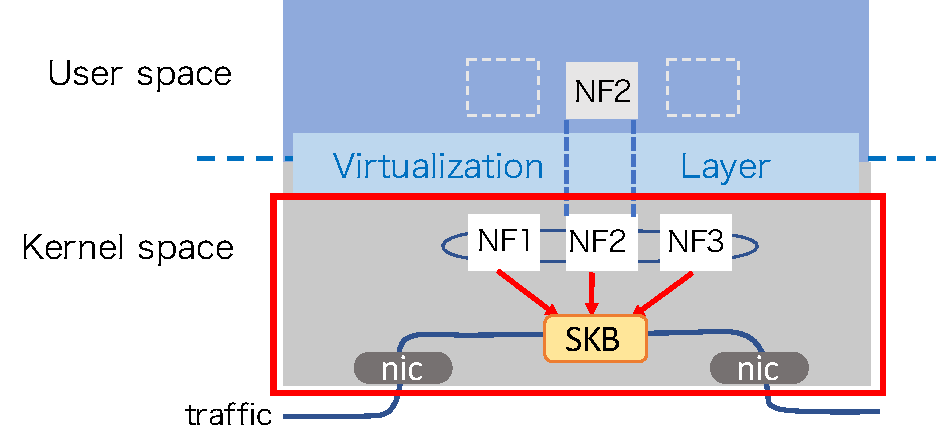
\includegraphics[width=95mm]{pics/path_kernel.pdf}
	\caption{Traffic in Kernel-based NFV node}
	\label{fig: path_kernel}
\end{figure*}

\section{Proposal: Lightweight NFC mechanism in Linux Kernel}
Because of the above two reasons, overheads in data path and resource consumption, I propose Kernel-based NFCI. Its aim is to realize lightweight NF chaining as much as possible in the kernel space on a single host. Simple and low load NFs should be executed in the kernel and NFs that require complicated tasks (e.g., tasks using encryption libraries) have to be put in the user space. The scope of this paper is the chaining mechanism for former NFs inside the kernel.

NF consists of one or more kernel modules. In order to integrate NF in network stack and manage traffic flow, I use Netfilter subsystem in Linux. Netfilter is a set of hooks inside the kernel that allows kernel modules to register its functions. A registered function is called for every packet that traverses respective hook within the network stack. The NF chaining takes place in the first hook before the routing decision. 

As Figure \ref{fig: path_kernel} shows, in my kernel-based NFCI node, NFs in kernel can directly access to the SKB because they are all in the same memory region. Hence there is no need of memory copy. When a NF cannot be completely executed in the kernel, only the simple function is placed in the kernel and scheduled by the well-tuned scheduling algorithm in Linux kernel, e.g., Completely Fair Scheduling (CFS)\cite{CFS}. The rest must be put in user space by a virtualization technology to be targeted for resource isolation. Because only complicated function is virtualized, overall resource consumption should be also decreased significantly. 

Certain amount of NFs consists of fairly simple functions, e.g., hash-based signature comparison and counting the number of specific flows,  and lots of them are feasible in the kernel. By providing a chaining mechanism for lightweight NFs in the kernel, overheads discussed so far will be largely eliminated. 

The structure of the thesis is as follows. Related work is introduced in Chapter 2. In Chapter 3, the overall picture of the Kernel-based NFCI is described. Chapter 4 describes the architecture of the Kernel-based NFCI. In Chapter 5, the detail of the implementation is explained. Results of the evaluations are shown in Chapter 5. And finally, I conclude this thesis in Chapter 6. 













\chapter{関連研究}
\label{chap:related}
\section{ETSI (European Telecommunications Standards Institute)}
ETSI\cite{ETSI} is a standardization organization in the telecommunications industry. Telecoms networks contain a large number of proprietary hardware and launch of new services often relied on on-site installation. In order to realize more flexibility for providing services ETSI proposed the NFV concept in 2012. Figure \ref{fig: ETSI_arc} shows the NFV architectural framework. The right box with dotted line represents the control plane and bigger box in the left with virtualized NFs atop describes NFV infrastructure installed in data plane. There is virtualization layer and virtual instances to support NFs because VM is used to realize NF. Detailed architecture is explained in the 2.2 section. 

\begin{figure*}
	\centering
	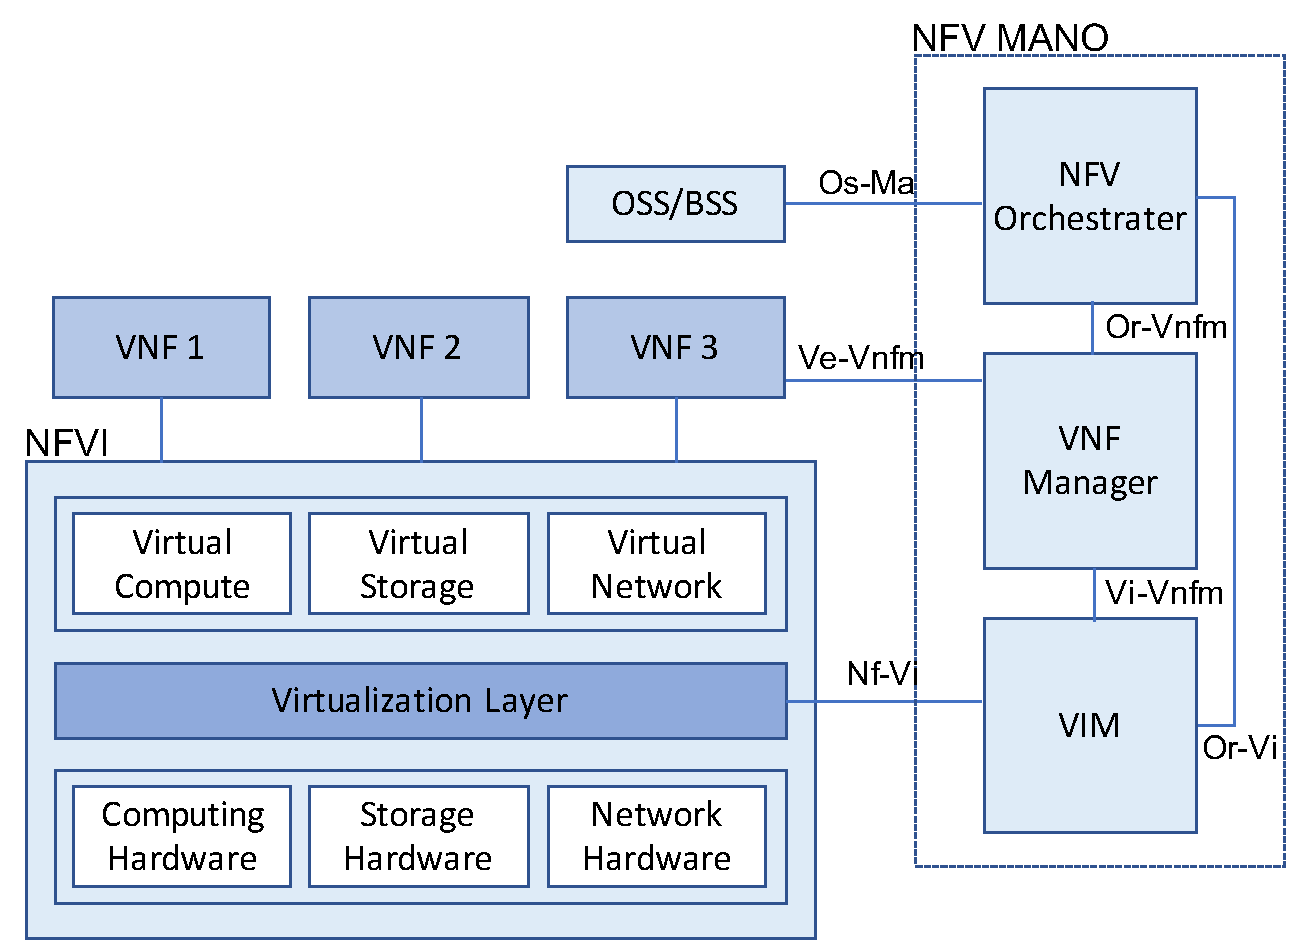
\includegraphics[width=100mm]{pics/ETSI_architecture.pdf}
	\caption{Architectural framework of NFV by ETSI.}
	\label{fig: ETSI_arc}
\end{figure*}

\section{OPNFV --- Open Platform for NFV}
\subsection{OPNFV: Architecture}
OPNFV\cite{OPNFV} is an open source project that realizes the architecture proposed by ETSI to provide carrier-grade, integrated platform for NFV. The OPNFV software platform is comprised of lot of projects and components related to NFV technologies. The architectural framework consists of the following 5 components. 
\begin{enumerate}
	\item Virtualised Network Function (VNF): One VNF may consists of multiple VMs, or in other cases, the whole VNF can be realized in a single VM.  
	\item Network Functions Virtualization Infrastructure (NFVI): NFVI has hardware and software part. Hardware NFVI corresponds to physical hardware such as servers, storage and network hardware. Software NFVI has 3 elements. First, virtual compute element which provides datapath for running VMs such as KVM. Secondly, virtual network element such as OVS, and thirdly virtual storage. 
	\item Virtual Infrastructure Management (VIM):  VIM controls and manages the interaction of a VNF with virtual compute, storage and network, as well as their virtualization. More specifically, it is in charge of allocating/releasing VMs on the hypervisors, increasing/decreasing resources to VMs. OpenStack, one of the largest open source projects in the world, is used as VIM in OPNFV. OpenStack itself is an umbrella project, containing numerous projects underneath. For example, Nova project for virtual compute service and Cinder project for virtual storage service are used in OpenStack.
	\item NFV Management and Orchestration (MANO) : Decoupling VNF from the underlying hardware resources requires an orchestrater that manages virtualization-specific tasks. It includes instantiating VNFs at appropriate locations, allocating hardware resources to the VNFs, keeping track of VNF instances location, etc. MANO is responsible of managing NFV infrastructure as described above to realizing network services. Following components manage virtual compute, networking, storage and VM resources. 
		\begin{itemize}
			\item NFV Orchestrater: Responsible for loading new network services and monitoring its lifecycle, and global resource management. As in Figure \ref{fig: ETSI_arc}, NFV orchestrater has interface between VNF Manager, VIM and OSS/BSS (Operation Support System / Business Support System). The first Or-Vnfm interface is used for VNF Manger to request virtual resources, and for NFV Orchestrater to send configuration information to VNF Manager so that VNF can be configured according to network service's demand. Or-Vi interface sends resource reservation/allocation requests by NFV Orchestrator. OSS/BSS is an interface that service provider operates through. 
			\item VNF Manager: Monitors lifecycle of VNF. Vi-Vnfm interface conveys resource allocation requests by VNF Manager to VIM. Ve-Vnfm interface is used for VNF lifecycle management and exchange of state information. 
		\end{itemize}
	\item Software Defined Networking (SDN) Controller: (SDN) Controller is control plane that is responsible for programming physical and virtual networking elements. SDN controller has northbound interface that connects with MANO and VIM, and southbound interface to physical and virtual networking switches. One of the southbound interface that is used is OpenFlow, which defines the communication protocol to enable SDN controller to directly interact with the forwarding plane. 
The aim of SDN controller in OPNFV is to set up overlay networks that connects VMs, so that NF chaining is accomplished. SDN controllers such as OpenDaylight\cite{OpenDaylight}, OpenStack Neutron and ONOS are integrated in OPNFV.
\end{enumerate}

A Network Service is described as a NF Forwarding Graph in OPNFV. NF Forwarding Graph has NF nodes connected with virtual link and underlying physical nodes connected with physical link. Figure 4 depicts an example of NF chaining. Forwarding Graph is composed of NF, VNF1, VNF2, ..,VNF4. Depending on the flow, traffic can go through NF chaining of NF1, NF3, NF4 or NF1, NF2, NF4. 
\begin{figure*}
	\centering
	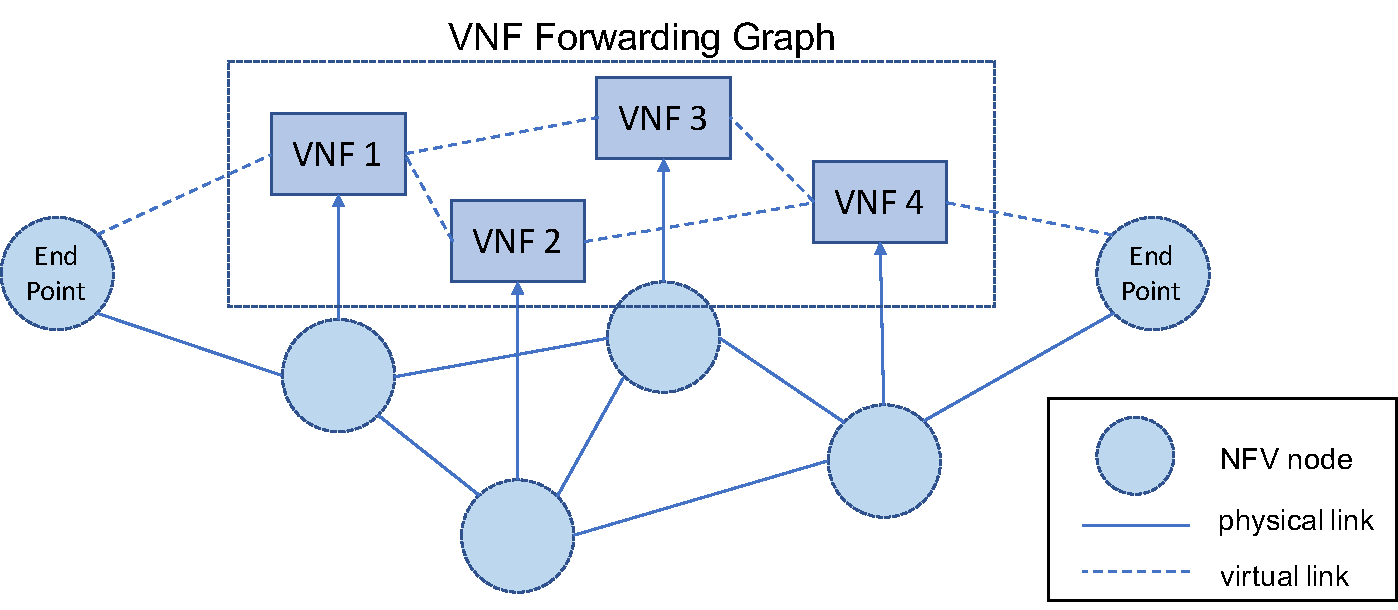
\includegraphics[width=120mm]{pics/NFV_FG.pdf}
	\caption{NFV Forwarding Graph}
	\label{fig: OPNFV_FG}
\end{figure*}

\subsection{Disadvantages of OPNFV}
Although OPNFV is a NFV platform that is widely deployed by enterprise and service provider, this thesis states the following two problems.
\begin{itemize}
	\item Complexity of OPNFV \\
		The architecture of OPNFV contains numerous middleware like OpenStack as a cloud controller, OpenDaylight as a SDN controller, KVM as virtual technologies, etc. Each of them are deriving from different project. This makes the architecture to be complicated and thus prone to compiling errors in different environments. 
	\item Resource consumption \\
		By allocating virtual instances to each of the VM, it leads to a lot of resource consumption when deploying a large number of VMs. 
	\item 
	\item Scaling problem of OPNFV \\
		OPNFV uses NFV Forwarding Graph to achieve NF chaining. SDN controller like OpenDaylight installs flow classifier in each NFV node. And OVS in NFV node forwards traffic according to the installed classifier, such as passing packets through NF on its node or transmitting packets to another node. Since a SDN controller is responsible for setting up service chain, it is not realistic to be deployed in wide area network. 
\end{itemize}





\chapter{Overview of Targeted Network Functions}
\label{chap:overview}
\section{Necessity of in-kernel NF chaining}
The original Internet protocol suite TCP/IP was standardized in the 1970s and the TCP/IP stack was first implemented in BSD OS in the early 1980s. Since then lots of efforts were made to implement this protocol in other platform like Linux. At first mutual communication via the Internet was only leveraged in military and commercial use. But as the Internet grew bigger and network application such as file sharing among distant entities gained popularity, the networking function by TCP/IP became a "commodity service". This means that the availability of this protocol is demanded by the majority of normal users and therefore it became an essential component in the kernel. 

 38 years after the first implementation of network stack in kernel (BSD), demands against networking function has also progressed. Kernel now supports not only TCP/IP but also a lot of other protocols and simple per packet network function such as Firewall or NAT. They are implemented by Netfilter subsystem in Linux kernel. One of the recent trends in network industry is, as mentioned, Network Function Chaining and this is realized either by traditional proprietary hardware or virtualization technology. I believe that this NF chaining system should be implemented in the kernel of general purpose OS, likewise network stack was integrated in kernel decades ago. Even though there are certain number of advanced NFs that are required by network nodes and certain users, the only way to run them (except buying expensive dedicated hardware) is with the help of virtualization technology, which causes heavy resource consumption to make virtualized instances and unnecessary memory copy to apply functions to packets. That is why I propose NF chaining mechanism in the kernel space. The mechanism aims to realize the chaining of NFs that are not executable by the existing Netfilter subsystem in the Linux kernel. 
 
 However I do not think that all kinds of advanced NFs can work within the kernel space. In Sections 3.1.1 and 3.1.2, functions that organize NFs are categorized and typical example of executable NFs in kernel space and other NFs that cannot be configured in kernel space are listed. And in Chapter 3.2, the contribution of kernel-based NFCI node in Wide Area Network (WAN) is described. 
 
 \subsection{Categorization of Network Functions}
 Functions in NFs are categorized into two types:
 \begin{itemize}
 	\item Simple functions: NFs often include functions like read/write of the packet headers or read of application message. The former process is already realized by Netfilter for NF such as NAT. The latter process is for example used to inspect the content of the message (application payload). The mean of inspection determines whether it is feasible in the kernel or not. If it is a  process such as hashing the payload to compare with a value or understanding the application-specific protocol, it is categorized in this simple functions. The detail of the NFs that have such functions are described in the Chapter 3.2. 
 	\item Complicated functions: When addressing application payload in NF, dedicated libraries are sometimes used for sophisticated service. This often requires a lot of calculation and it is not suitable to place such function in the kernel. It is because if the process gains the highest priority, it will most likely takes up all the CPU time according to the Complete Fair Scheduling (CFS) in Linux. Therefore they should be virtualized and put in the user space to guarantee the isolation of resource like CPU. 
 \end{itemize}
 This thesis argues that simple functions described above are regarded executable in kernel space.

\subsection{Example of Network Functions and its Realizability in Kernel}
NFs are roughly divided into the following two categories. One is kind of NFs that need to work on the requesting node to provide the service, being security related functions like firewall. In the point that security measures that are more sophisticated than simple firewall will be essential for the majority of users, this kind of NFs are defined as commodity service in this thesis. And another kind is NFs that are to be placed on network nodes to provide better performance in overall network, such as Traffic Engineering (TE). 
\begin{itemize}
	\item Network Functions of Commodity Service\\
		Although NFs such as Firewall and NAPT which can check up to transport layer (Layer 4) are already implemented in Linux, NFs that require information that resides higher than Layer 4 are not. As example of latter NFs, there are Web Application Firewall (WAF) and Application Layer Gateway (ALG). 
		\begin{itemize}
			\item WAF\\
				WAF is a security control to protect web applications against attacks that traditional firewall could not prevent, such as SQL injection and cross-site scripting. WAF detects the threats by examining incoming HTTP traffic. Specifically, it analyzes all HTTP requests (GET and POST requests) to apply defined rules to identify malicious traffic. Set of signatures that represents patterns that are components of well known attacks are used against traffic payload. A pattern match of signature and the traffic payload means that it's illegal traffic.
			\item ALG\\
				ALG is a firewall for specific application protocols such as SIP (Session Initiation Protocol) and FTP (File Transfer Protocol). ALG acts an middlebox between the client and application server and controls whether to allow or deny traffic to application server. It recognizes application specific commands in application message and offers security controls over them. 
		\end{itemize}
	
		In the case of WAF, pattern matching of signature is what is basically done. Pattern matching can be checked against the whole message of a packet or only the first few tens of kilobytes of the message. The first case may require specific libraries and complex calculation and thus is not pragmatic to implement in kernel space. But in the second case, only the first part of the message will be hashed and this value is checked against the signature. Comparison of a hashed value is a simple process that also kernel module of OVS conducts when searching the flowtable. So the latter is feasible to implement in kernel and therefore is subject to my NF. 
		
		In the case of ALG, it is necessary to understand the application-specific protocol. For example in FTP, a command ``GET" can be placed in application payload to get file from the server. To recognize the complete message of the application, it is necessary to see the whole message. For example in case of TCP/IP, the IP stack that get data from application process will chop off the data to be sent up to the Maximum Segment Size (MSS), put them in TCP segments and then encapsulate them in IP packets. In order to get the original message before it was divided by MSS, TCP segments need to be reassembled. Since Netfiler only supports NFs that process per packet, it is yet not realized in Linux. Reassembling packets in the kernel space to realize the NF such as ALG is my future work.
		
	\item Network Functions of TE\\
		TE is a method for optimizing the performance of carrier network by dynamically analyzing and regulating the behavior of the data transmitted over the network. Representative NFs of TE is Multipath Routing and Network Caching. 
		\begin{itemize}
			\item Multipath Routing\\
				Mulitpath Routing supports multiple paths for a transmission of streams of data between two end points. This provides better utilization of available bandwidth, higher fault tolerance and load balancing over available resources. The process works as follows: All available paths to the destination is aggregated into a single virtual path. Packets from the applications are gathered to this virtual path and they are distributed to the actual physical path via mechanism such as round-robin or weighted fair queuing. By offering packets to all paths, available bandwidth can be fully utilized and even in the case of link failure streams can reach the endpoint continually.  
			\item In-network Caching\\
				Large percentage of web traffic consists of much of the same requests to web servers. These identical traffic can be significantly reduced by network caching technology. It keeps frequently accessed web content in a cache storage close to the requesters. The process works as follows: A user accesses a web page. If the local cache storage has the cache of the requested content it will be transferred to the user without the trouble of accessing the web server. Otherwise the local network cache get the content from the web server to store in the storage so that the next requester can use the cached content. 
		\end{itemize}
		These TE functions are also targeted NFs in the kernel-based NFV in the future. 
\end{itemize}

\section{NFC in WAN Environment} 
\subsection{Assumed Environment and Usage Model}
In WAN, there are companies as Network Service Provider (NSP) and Internet Service Provdier (ISP). NSP owns networking hardwares such as routers and switches (network node) that build up network infrastructure and sells network resources as bandwidth to ISP. And ISP provides the network resources to users. My future vision is that hardware routers or switches will be replaced by general purpose OS, and in that case kernel-based NFCI plays the roles of network node as well as normal user node. This means that basic NF chaining would be executed on each of network or user node by Kernel-based NFI without deploying virtualization technology. 

Depending on the kind of the NF, the place where the NF should be loaded is determined. For instance security related NF such as firewall and  WAF should run in the requesting user node. On the other hand, TE related NFs, load balancer, and so on are placed by NSP on network nodes. In both cases, a NF that is sent from the NSP is source code of kernel modules that makes up the NF. The kernel modules will be then compiled in the environment of the installed node and start to function. Figures \ref{fig: overview_1} and \ref{fig: overview_2} show the placement of the two kinds of NFs in WAN. It is assumed that Network nodes and user nodes are operating on Kernel-based NFCI. 

\begin{figure}[htbp]
	\begin{minipage}{0.5\hsize}
		\begin{center}
			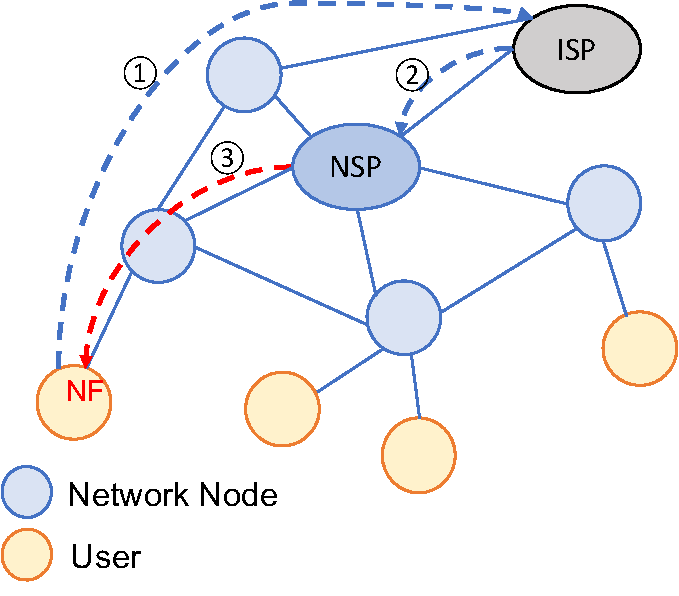
\includegraphics[width=75mm]{pics/overview_1.pdf}
		\end{center}
		\caption{NF request by user}
		\label{fig: overview_1}
	\end{minipage}	
	\begin{minipage}{0.5\hsize}
		\begin{center}
			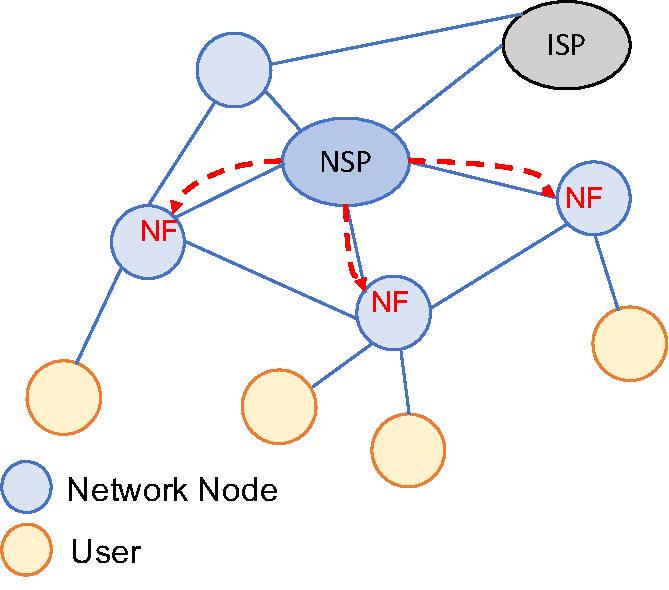
\includegraphics[width=75mm]{pics/overview_2.pdf}
		\end{center}
		\caption{NF placement by NSP}
		\label{fig: overview_2}
	\end{minipage}	
\end{figure}

Figure \ref{fig: overview_1} explains process where the former NFs are loaded. 1) User node requests a NF to ISP. 2) ISP then tells the NSP where to load the requested NF, in this case in the requesting user node. 3) NSP loads the NF in the right node. 

Figure \ref{fig: overview_2} depicts the case of latter NFs placement. These NFs are not requested by user nodes but the NSP itself loads them in network nodes. This is because latter NFs such as TE related ones contribute to the overall higher performance in networking such as better utilization of bandwidth and hence producing more profit for the company. When the NSP decides that the traffic between user A and user B should pass through a NFs of this kind, there are two ways to realize this. The first way is to load necessary NFs in network nodes on the shortest path between users. The second way is to user Network Service Header (NSH\cite{NSH}) to change the path of the traffic to traverse network nodes that already installed NFs in demand. 

	\begin{itemize}
		\item Loading on shortest path\\
			The former way is easier to do in terms of no need of modifying the path. But it is not hard to imagine that this will leads to redundant placement of NFs in network nodes. As each time a new traffic flow has to be processed by NFs, it is likely that the same NFs will be placed in different network nodes. 
		\item NSH\\
			NSH is added in each packet header as an information of designated service function path in a single administrative domain. NSH describes a sequence of service function nodes that the packet must be routed prior to reaching the destination. NSH is inserted between the original packet and outer network encapsulation such as MPLS, VXLAN, etc. Important information is placed in service path header in NSH. It consists of 24 bits of Service Path Identifier (SPI) and 8 bits of Service Index (SI). SPI identifies service function path and SI is an indication of number of processed service function. 
			
			Network function chaining by NSH requires the following three components: control plane, Service Classifier (SC) and Service Function Forwarder (SFF). As in the figure \ref{fig: NSH} , there is ingress and egress routers in the network marked with SC and network nodes with SFF and SF. Control Plane is in charge of creating service chain and setting the regarding information in SCs and SFFs. 
			
			As a packet enters ingress router, SC classifies the packet according to the pre-defined policy and apply NSH to the packet with appropriate SPI and SI value. And the packet is sent to the next hop to be processed by FSS. FSS determines the forwarding destination for the first SF based on the NSH and insert overlay header (e.g., VXLAN header) for transmission. When the packet arrives at the SF, the overlay header is striped and the SF takes action. Subsequently SI value is decremented by one and FSS applies new NSH and overlay header to transmit to the next SF. When the service function chaining completes, NSH will be removed at egress SC and normal forwarding resumes.   
			
			The advantage of NSH in comparison with OpenFlow-based network operation is the scalability. To use OpenFlow for programming NF chaining, it is necessary to set up all the nodes in the network with OVS. OpenFlow uses Match-Action flowtable which directs packets regardless of the shortest path. If there is a node that does not understand OpenFlow in the same network it could cause loop in the network. So OpenFlow can be used in a single datacenter network or interconnection between small-scaled datacenters in the biggest use case. On the other hand, NSH does not require all the nodes to be NSH-aware. Only the nodes that host Service Functions and ingress/egress routers should understand NSH protocol. This is because the routing from a FSS to the next FSS is done by overlay network so that non-NSH-aware nodes between them can route the packet with shortest path policy. When using NSH, configuring NF chaining in large scale network between datacenters is also possible. From those reasons, NSH is the technology that we want to use for Kernel-based NFV in the future. 
	\end{itemize}
	
\begin{figure*}[t]
	\centering
	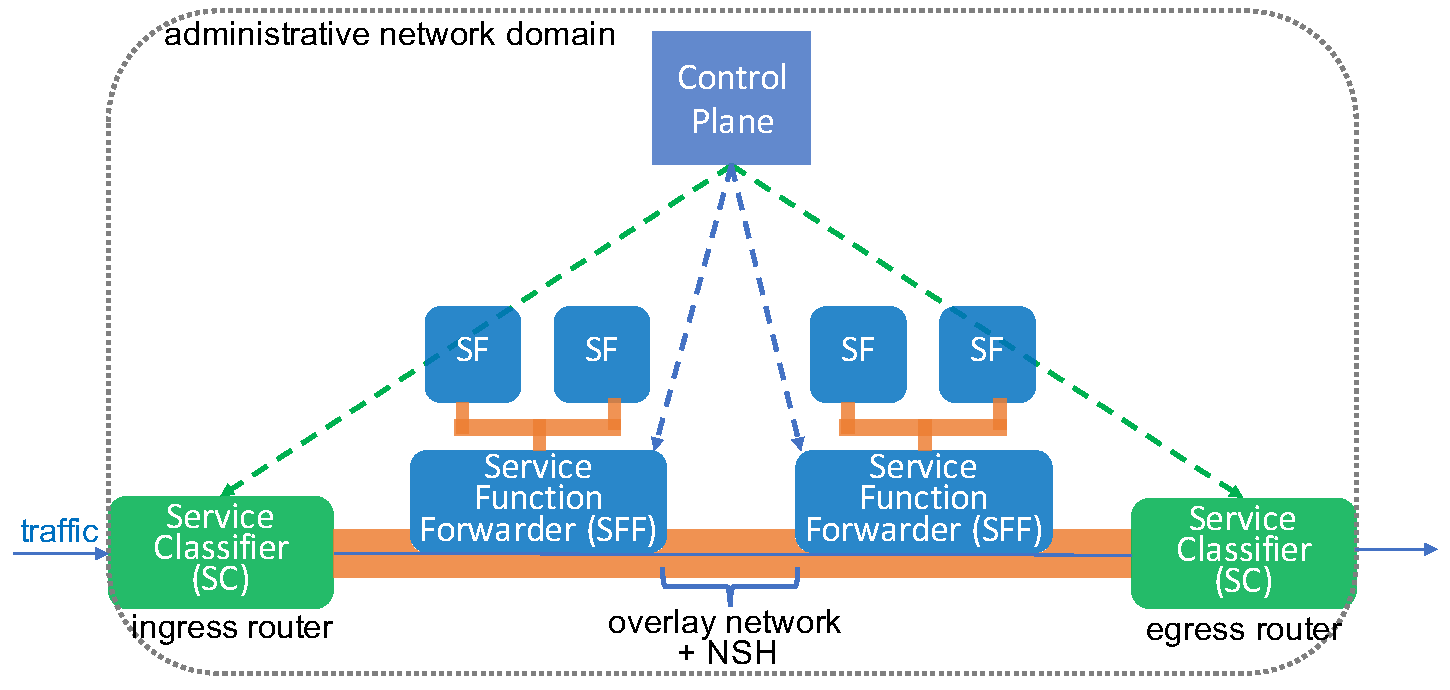
\includegraphics[width=120mm]{pics/NSH.pdf}
	\caption{NSH Architecture}
	\label{fig: NSH}
\end{figure*}

\subsection{Scope of the paper}
This thesis focuses on the data plane of NF chaining rather than control plane.  Specifically, NF chaining mechanism for per packet process in a single host is implemented. The system of reassembling IP packets to acquire the original payload for NF such ALG remains as future work. 












\chapter{Netfilter Subsystem in Linux Kernel}
\label{chap:linux}
The proposing Kernel-based NFCI makes use of existing Netfilter subsystem in Linux kernel. In this chapter detailed description about this Netfilter subsystem is given. 

\subsection{Netfilter: Overview}
Netfilter is a software inside the Linux 2.4.x and later kernel series, which enables packet filtering and packet mangling. It is a set of hooks that are placed in several stages in network stack and in each hook multiple kernel modules can be registered. Each of the kernel module will work as a NF, such as Firewall and NAPT. 
Figure \ref{fig: netfilter_system} shows the network stack and five netfilter hooks embedded inside it. The bottom is the device driver and the more it goes up the network layer does as well to reach the transport protocol (Layer 4). As packets progress through the stack, the registered kernel modules in the hook will be triggered. 
The following hooks are located in meaningful positions in the stack:
\begin{itemize}
	\item PRE\_ROUTING : This hook is triggered by incoming packet soon after entering the network stack. This is processed before the packet reaches the routing subsystem.
	\item LOCAL\_IN : This hook is processed after the packet has been routed and is destined to the local host.
	\item FORWARD : This hook is processed after the packet has been routed and is to be forwarded to another host. 
	\item LOCAL\_OUT : This hook is triggered by locally created packet as soon as it enters the stack.
	\item POST\_ROUTING : This is the last hook that the outgoing or transmitted packet passes before being put out on the wire. 
\end{itemize}

\begin{figure*}
	\centering
	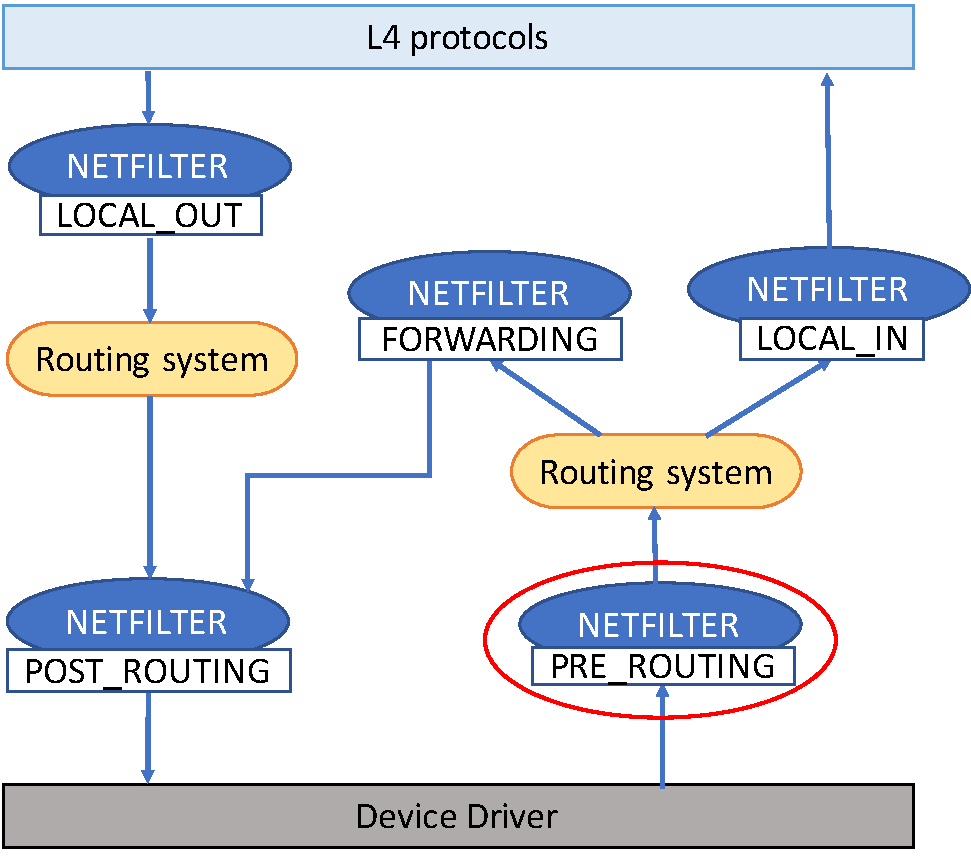
\includegraphics[width=90mm]{pics/netfilter_system.pdf}
	\caption{Netfilter hooks in network stack}
	\label{fig: netfilter_system}
\end{figure*}

Kernel modules that are registered in a hook according to the its priority. The lower the priority value is, the earlier it gets executed. Each kernel module will return a verdict indicating the result of the process. 

\subsection{Netfilter: Table}
Netfilter supports Firewall, NAPT and so on. Each of these NF has its own "Table" to organize the rules. Rule is used to specify which kind of flow is targeted for the specific action, such as filtering in case of Firewall. In each netfilter hook, the following tables can be registered. 

\begin{table}[tb]
	\centering
	\caption{List of tables in Netfilter hooks}	
	\begin{tabular}{|c|c|c|c|c|c|}
		\hline
		\backslashbox{Tables}{Hooks} & 	PREROUING & INPUT & FORWARD & OUTPUT & POSTROUTING \\
		\hline
		\hline
		Mangle & $\bigcirc$ & $\bigcirc$ & $\bigcirc$ & $\bigcirc$ & $\bigcirc$ \\
		\hline
		CT & $\bigcirc$ & & & $\bigcirc$ & \\
		\hline
		DNAT & $\bigcirc$ & & & $\bigcirc$ & \\
		\hline
		Filter & & $\bigcirc$ & $\bigcirc$ & $\bigcirc$ & \\
		\hline
		SNAT & & $\bigcirc$ & & & $\bigcirc$ \\
		\hline
	\end{tabular}
\end{table}

\begin{itemize}
	\item Mangle Table : Mangle Table is used to alter the IP headers of the packet in various ways. For instance, one can adjust the TTL value of a packet to either lengthen or shorten the number of network hops. 
	\item Connection Tracking Table (CT) : CT enables stateful operation by associating packets with a connection. CT checks each packet against existing connections. If the first packet of a new flow enters the system, a new connection will be created. Otherwise the state of the connection will be updated accordingly. Only CT can be used, for example allowing only packets that are associated with an established connection. It is also common to use CT with NFs that want to see the packets in the context of an ongoing connection. NAPT is one of the such NF that make use of CT.
	\item DNAT / SNAT Table : NAT is divided into two DNAT and SNAT. DNAT is responsible of changing the destination IP address or port, whereas SNAT changes source IP or port. DNAT table can be placed in PRE\_ROUINTG and OUTPUT hooks, both before the routing subsystem because the change of destination part would change the routing decision as well. Meanwhile SNAT takes place at LOCAL\_IN and POST\_ROUTING, both before being delivered to the destined host. 
	\item Filter Table : The filter table is used to make decision about whether to allow packet to continue to its destination or drop the packet. Unlike the above tables, when a rule matches only a verdict whether to accept or drop is returned without doing any specific process. This is normally used for Firewall for filtering mechanism. 
\end{itemize}

\subsection{Netfilter: Rule and Target}
In each table a sequence of rules are installed, which forms a "chain of rules". The rules will be evaluated from top to down in the chain. A rule is registered with a target component, which has function or verdict. Any target returns integer value named verdict which determines how the packet will be handled.
 The verdict value XT\_CONTINUE and XT\_RETURN are special. When the verdict is XT\_CONTINUE the next rule in the chain is further evaluated. And XT\_RETURN means to jump to another rule chain. The other main verdicts are NF\_ACCEPT, NF\_DROP. NF\_DROP tells to discard the packet. NF\_ACCEPT means that the traversal of rule chain terminates in the table and the packet will be further processed by the next table if any or return from the netfilter system to the network stack. 
 
There are following cases when a rule matches: 
\begin{enumerate}
\renewcommand{\labelenumi}{\arabic{enumi})}
	\item Only a verdict (NF\_ACCEPT, NF\_DROP, etc.) gets returned without doing any process.
	\item Registered function in the target is executed and returns verdict according to the result of the process.
	\item Jump to another rule of chain. 
\end{enumerate}

Figure \ref{fig: ip_chains} shows an abstract image of traversal of rule chain. 

Rule Chain0 and Rule Chain1 belong to the same table. Smaller boxes in the rule chains represents sets of rule and target. A packet will be evaluated from the top of rule chain until the target's verdict returns NF\_DROP or NF\_ACCEPT. Suppose we get a TCP packet with destination port X and destination IP y.y.y.y and we need to process it through firewall table in figure \ref{fig: ip_chains}. The packet enters rule chain0 for screening and first checked against "UDP port = Y" rule. Since the first rule doesn't match, it proceeds to the next rule "proto = TCP". The second rule matches and therefore the target is executed. The target is a verdict "XT\_RETURN" so the packet jumps to another chain, in this case Rule Chain1 for further screening. The first and second rule in rule chain 1 both don't match so the packet jumps back to the rule chain0 to start from the third rule. The third rule matches so the target  which is a function in a registered kernel module is executed. This function1 returns verdict and if the verdict is either NF\_DROP or NF\_ACCEPT, the screening in this table terminates. If the verdict is XT\_CONTINUE then it continues to the next rule. The last evaluated rule's target decides the verdict of the packet. 

\begin{figure*}
	\centering
	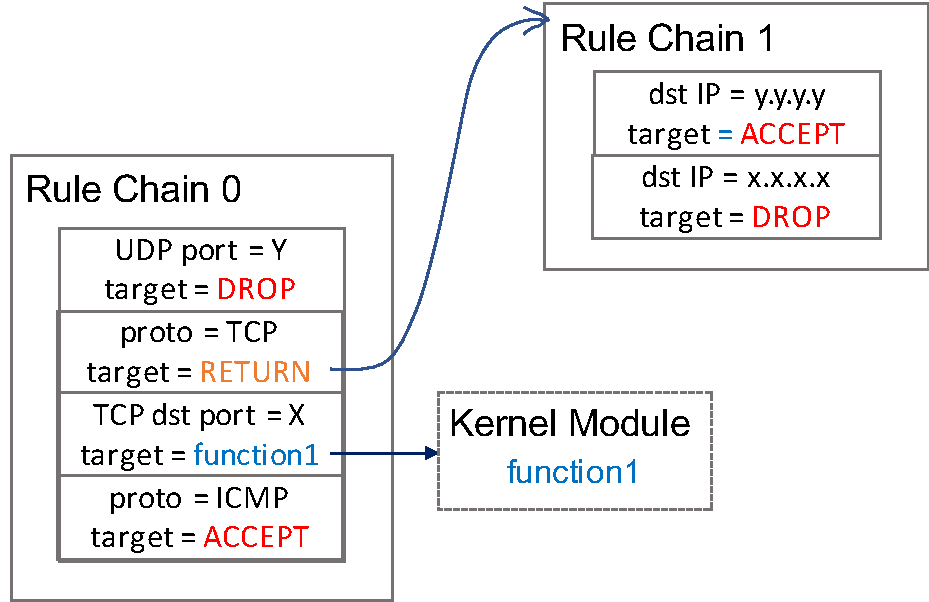
\includegraphics[width=90mm]{pics/ip_chains.pdf}
	\caption{Ipchains rules and targets}
	\label{fig: ip_chains}
\end{figure*}




\chapter{Kernel-based NFCI Architecture}
\label{chap:architecture}
In this chapter, detailed description of NF chaining mechanism in kernel space is given. 

The design of the Kernel-based NFCI is shown in Figure \ref{fig: design}. All the arrived packets are first checked by the registered rules that determines which flow should be processed by which NF chain. If the packet matches a rule the corresponding NF chaining starts. The NFs in the chain are executed in registered order. Each NF processes packets by directly accessing with pointer. 
 
 \begin{figure*}
	\centering
	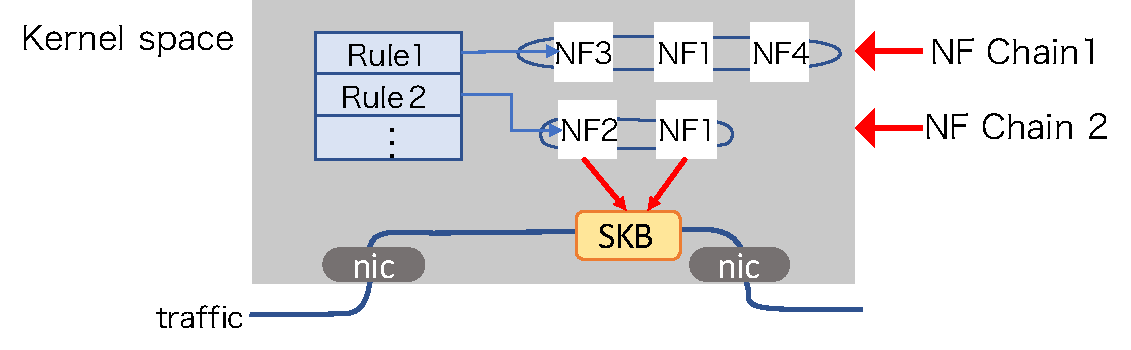
\includegraphics[width=120mm]{pics/design.pdf}
	\caption{Design of the Kernel-based NFCI.}
	\label{fig: design}
\end{figure*}

Kernel-based NFCI has three main components. One is the identification of flow. The second is chaining of NFs, the system that enables packets to be processed by NFs in order. And the last is the NFs themselves. Any kind of NF consists of one kernel module or more. The NF chaining mechanism takes place in the PRE\_ROUTING hook which locates between hardware and routing subsystem in the network stack, which is called here chaining point. 

\section{Network Function}
Any installed kernel modules exist in the same memory region as kernel so the functions in the modules can be seen from other modules and from kernel. This is why it is possible to call functions in kernel modules from network stack. Normally a NF consists of several kernel modules. And in this case, the very first function among kernel modules should be registered somewhere in the kernel and the subsequent functions in other kernel modules will be called in order. 

\section{Identification of Flow}
In the kernel-based NFV host, sets of NF chain can be registered. When a network node participates in NF chaining, it is likely that many flows comes in and out. Not all the flows are to be processed by a single NF chain but only specific flows should pass its designated NF chains. So a mechanism is needed to specify which kind of flow should be treated by a chain of NFs in the host. For example in OPNFV, OVS is used to direct flows to the right NFs which are in VMs. OVS employs OpenFlow which can set a very detailed rules using VLAN tag, incoming / outgoing port, etc. Kernel-based NFV distinguishes flows in granularity of five tuples. Five tuples represent source / destination IP address, source / destination port number and the transport protocol. 

The identification of flow in 5-tuple is implemented using Filter table. As explained in Sec. 4.1.2, Filter table carries out filtering by setting rule and verdict of NF\_DROP or NF\_ACCEPT. Instead of setting verdict in the target, pointer to the list head of chained NFs is registered. 

\section{Chaining of Network Functions}
This mechanism uses Doubly Linked List (DLL) to implement NF chaining. DLL is a list that contains links to next and previous nodes. Unlike singly linked lists traversal is only one way, DLL allows traversal in both ways. 
Figure \ref{fig: dll} shows the framework of NF chain realized with DLL. DDL is chosen since adding and removing node can be done easily. A NF is represented by a node of gray box. A node is a {\tt nf\_target} struct which has the following members: 
\begin{itemize}
	\item {\tt list\_head} struct : {\tt list\_head} struct has two pointers, next and prev, which respectively points to the previous node and next node. 
	\item pointer to function : This points to the function in the kernel module. The function will execute the process of NF.
	\item priority : This is a integer value that is used to put the {\tt nf\_target} struct in the right position in the DLL. The smaller the value is, the higher the priority is.
\end{itemize}

\begin{figure*}
	\centering
	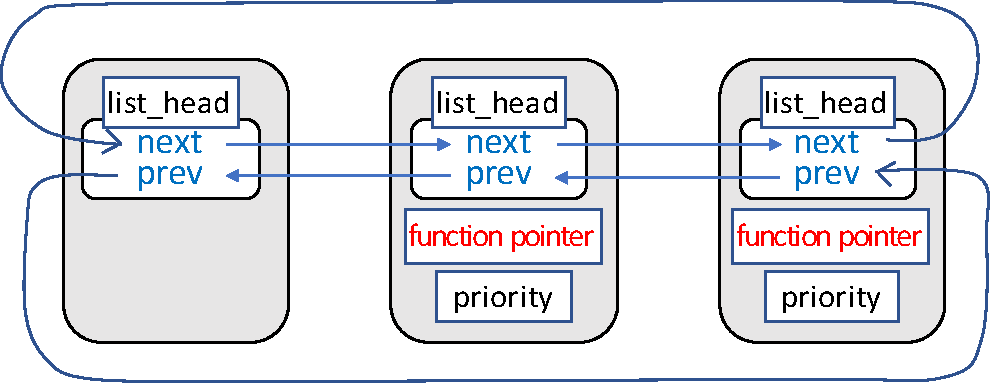
\includegraphics[width=90mm]{pics/dll.pdf}
	\caption{Doubly Linked List with nodes of {\tt nf\_target} struct.}
	\label{fig: dll}
\end{figure*}

\begin{figure*}
	\centering
	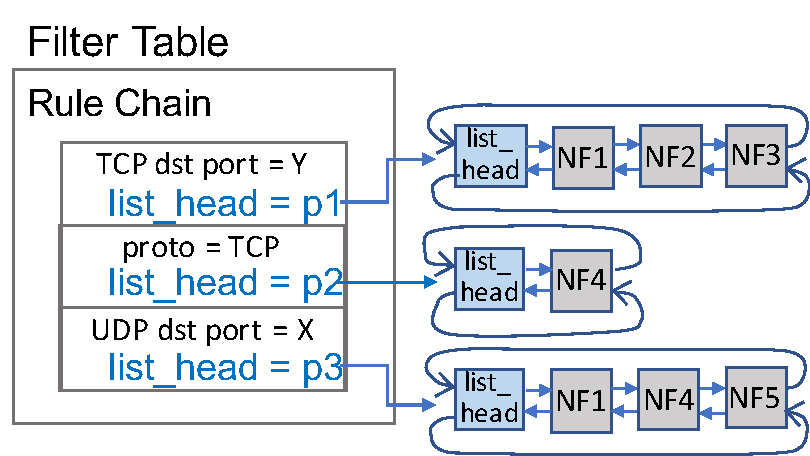
\includegraphics[width=90mm]{pics/list_head.pdf}
	\caption{Structure of rules and the corresponding NF chain in Filter Table.}
	\label{fig: listhead}
\end{figure*}

 When inserting a NF in a chain, the priority and the function to be registered must be given. According to this information and network namespace, a {\tt nf\_target} struct is created and inserted in the corresponding DLL. The struct is inserted before the node that has higher priority. 
 
 Figure \ref{fig: listhead} shows the example of Filter table and how the DLL that represents NF chain is linked. The mechanism that is responsible for NF chaining is called NFC system from here. When a packet arrives at the chaining point, it first traverses the Filter table to be passed to the right NF chaining. If a rule matches, the corresponding chaining starts: The NFC system takes the list head of the registered NF chain from the target component. Now from the next node in the DLL, which is the first NF, starts the process. The pointer to the SKB (Socket Buffer) is passed to the registered function in the node which will starts the entire the NF process. When the process is finished, the control comes back to the NFC system. At this point the function in the node returns verdict as well. There are only two types of them, DROP or ACCEPT. If it returns DROP, the NFC system stops the chaining and the SKB will be freed. Otherwise the system pass the SKB pointer to the function in the next node to process the next NF. The same procedure will continue until the last NF in the chain is executed. When the last NF returns ACCEPT, the NFC system ends NF chaining for the SKB and it will move to the next stage of network stack. 

As an example, when a UDP packet with destination port X arrives at the Filter table configured like Fig. \ref{fig: listhead}, the first and second NF chains are skipped. And the packet matches the last rule so the NF chaining of NF1, NF4 and NF5 starts. If all functions of NFs return ACCPET, this SKB that is probably modified by three NFs continues its journey in the network stack. 


\chapter{実装}
\label{chap:implementation}
\section{Implementation of NF chaining in kernel}
In this paper, I implemented the prototype of per packet NF chaining mechanism in the kernel space. This includes identification of flow, NF chaining system and implementation of two NFs, DoS attack denial and DNAT. 

\subsection{Environment of implementation}
For the implementation, VM is used running atop hypervisor. Ubuntu 16.04 LTS (64bit) is used as VM's OS. 

\subsection{Detailed structure of table}
As explained in the chapter 4.2.2, identification of flow is done with the help of Filter table. Usually the daemon in the user-space takes the command for iptables and set the specified rule in the kernel space. Instead of this, I made a kernel module that is responsible for inserting rule in the Filter table. 

Table is a contiguous memory region where rules and targets are inserted. Every network namespace (ns) has its own tables. Specifically, struct net that represents ns, has struct netns\_ipv4 member, which contains pointers to each table. All tables (from Filter to NAT table) are the same struct xt\_table. 	


Figure \ref{fig: filter_table} describes the Filter table. The xt\_table struct has ipt\_table\_info struct that includes pointers to the top of each hook's rule. For example, hook\_entry[0] in ipt\_table\_info points to the top of rule in LOCAL\_IN hook. And hook\_entry[1] points to the top in LOCAL\_OUT hook. To sum up, the biggest box in the middle row is the part of the Filter table for LOCAL\_IN hook and the below box is another part for LOCAL\_OUT hook and so the rest of part for other hooks continues. The box that starts with ipt\_entry and finishes with ipt\_entry\_target corresponds to a set of rule and target which were depicted by a small single box in Figure 4.2. 

\begin{figure*}
	\centering
	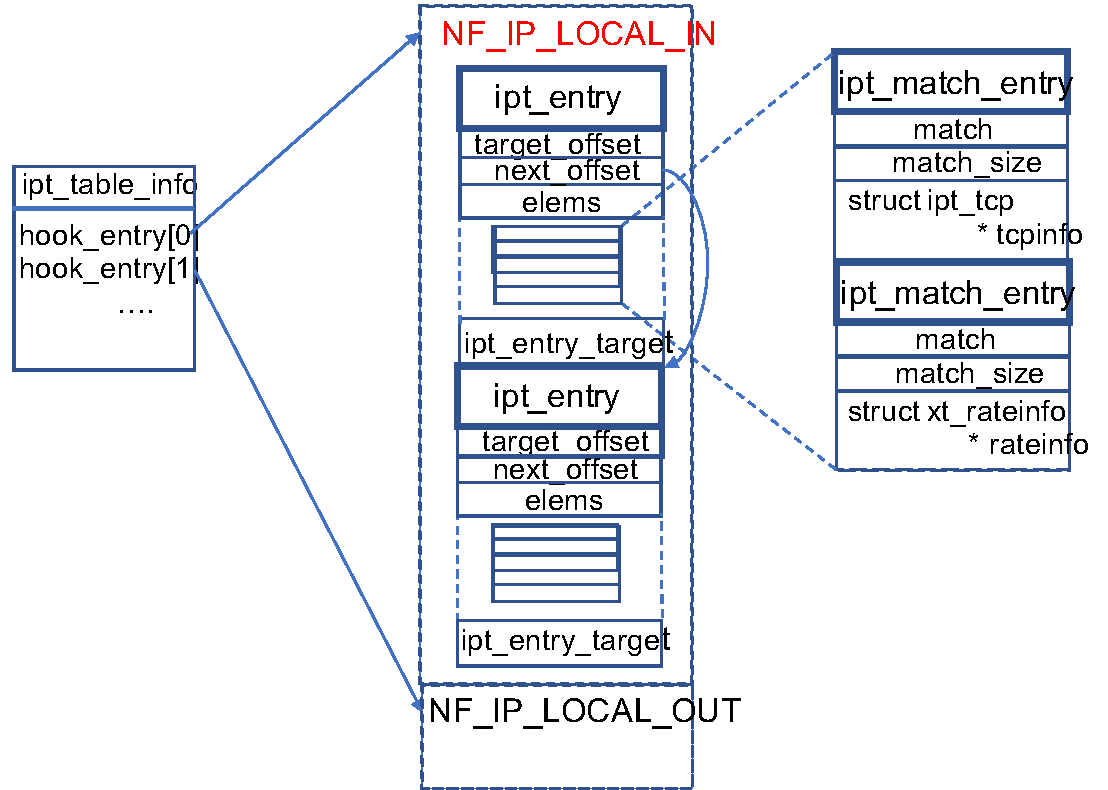
\includegraphics[width=140mm]{pics/filter_table.pdf}
	\caption{Filter Table}
	\label{fig: filter_table}
\end{figure*}

A rule is represented by the following ipt\_entry struct. The ipt\_ip struct member has in\_addr struct to store source and destination IP address of the rule. If no rule for IP address is specified, they are both initialized to 0.0.0.0. Also a protocol number is set in ipt\_ip struct. target\_offset is the offset to the corresponding target, ipt\_entry\_target struct. And next\_offset is the offset to the next rule, ipt\_entry struct. 

The last member elems[0] points to the top of protocol specific rules. A struct ipt\_match\_entry is used to insert specific rules for TCP, UDP, incoming/outgoing device, etc. Similarly to ipt\_entry\_target struct, ipt\_entry\_match struct has user struct and kernel struct inside a union. ipt\_match\_entry struct is organized as following:  In the struct xt\_match, a function pointer can be registered to check protocol specific part of the packet. For example, tcp\_mt function is registered to check TCP header, such as source / destination port number, TCP option and so on. To accommodate various protocol specific rule, data[0] is used. For example, TCP specific rules are inserted to ipt\_tcp struct and the pointer to this struct is assigned to data[0]. Likewise any protocol can be checked. 

Struct ipt\_entry\_target is where the information of action (target) against rule match is inserted. Inside ipt\_entry\_target, there is a union containing "user" struct and "kernel" struct. The former is used when the target has only verdict and no process to be executed. The latter is used when the target has function to  execute. Specifically, the xt\_target struct member contains the pointer to the function. In order to realize NF chaining, head of the chain "struct list\_head" is inserted as the last member. So the first two structs in ipt\_entry\_target is ignored and only the last struct list\_head member is used in case of NF chaining. 

\subsection{Preparation of NF chaining} 
There are two kernel modules that are responsible of preparing the NF chaining: The first "create\_nfc" module makes NF chains. The second is responsible of setting up rule in Filter table for a chain. Especially struct ipt\_entry (in figure \ref{fig: imp2}) and struct ipt\_entry\_target (in figure \ref{fig: imp3}) are used to set rule. 

Before create\_nfc module make a NF chain, kernel modules that forms each NF should be installed in advance. The following information must be provided from the NF : Pointer to the first function of the NF, its priority value, the name of the NF and identification number o f the desired chain (CI). According to this information create\_nfc module first of all makes a struct nf\_target as described in \ref{fig: imp1}. The provided function pointer is registered in the second member in struct nf\_target and so on. If CI is new, a new NF chain is created. Specifically, a new struct list\_head is allocated and the nf\_target struct is inserted as next node, forming a DLL. If CI already exist, the NF should be inserted in the appropriate existing chain. The priority value in the chain is examined and the the nf\_target struct is inserted before the node that has higher priority value.

This second module does roughly three things. 
\begin{itemize}
	\item Setting Rule for NF chain : A rule is set to specify which kind of flow should pass the corresponding NF chain. For IP related rules struct ipt\_ip member is set and for protocol specific rule struct ipt\_match\_entry that is pointed by elems[0] is set. 
	\item Setting the last rule : If none of the set rule for NF chaining matches, the packet will be discarded. To allow packets that is not intended to be processed by any NF chain to go through this system, the last rule is inserted. This rule matches any flow and the target is set as NF\_ACCEPT verdict. 
	\item Registering head of NF chain : After making DLL which forms a NF chain, the head of this DLL is assigned to list\_head member in ipt\_entry\_target struct. 
\end{itemize}

\begin{figure}
	\begin{center}
		\begin{screen}
			\begin{verbatim}
struct nf_target {
     struct list_head list;
     unsigned int (*nf_func)(struct sk_buff *skb);
     int priority;
     char name[20];
};
			\end{verbatim}	
		\end{screen}
	\end{center}	
	\caption{Struct nf\_target}
	\label{fig: imp1}
\end{figure}

\begin{figure}
	\begin{center}
		\begin{screen}
			\begin{verbatim}
struct ipt_entry {
     struct ipt_ip ip;          // IP related rule
     unsigned int nfcache;
     __u16 target_offset;       // Offset to the corresponding target struct
     __u16 next_offset;         // Offset to the next ipt_entry struct 
     unsigned int comefrom;
     struct xt_counters couters;
     unsigned char elems[0];    // Pointer to region of the protocol-specific rule 
};	
			\end{verbatim}
		\end{screen}
	\end{center}
	\caption{Struct ipt\_entry}
	\label{fig: imp2}
\end{figure}

\begin{figure}
	\begin{center}
		\begin{screen}
			\begin{verbatim}
struct ipt_entry_target {
     union {
            /* Used for user-space daemon to get info */
            struct {
                 __u16 target_size;            // Size of user struct 
                 char name[XT_EXTENSION_MAXNAMELEN];
                 __u8 revision;
            } user;
            /* Used for target with function */
            struct {
                 __u16 target_size;            // Size of kernel struct 
                 struct xt_target *target;     // Function to be executed 
            } kernel;
            __u16 target_size;                 // Size of ipt_entry_target struct 
     } u;
     unsigned char data[0];
     struct list_head *head;     // Pointer to the head of the corresponding DLL
};
			\end{verbatim}
		\end{screen}
	\end{center}
	\caption{Struct ipt\_entry\_target}
	\label{fig: imp3}
\end{figure}
			
\begin{figure}			
	\begin{center}
		\begin{screen}
			\begin{verbatim}
struct ipt_entry_match {
     union {
            /* Used for user-space daemon to get info */
            struct {
                    __u16 match_size;
                    char name[XT_EXTENSION_MAXNAMELEN];
                    __u8 revision;
            } user;
            struct {
                    __u16 match_size;
                    struct xt_match *match;
            } kernel;
            __u16 match_size;
      } u;
      unsigned char data[0];
};
			\end{verbatim}
		\end{screen}
	\end{center}	
	\caption{Struct ipt\_entry\_match}
	\label{fig: imp4}
\end{figure}

\subsection{Implementation pf NF chaining mechanism}
The PRE\_ROUTING hook is triggered at the end of ip\_rcv function (in net/ipv4/ip
\_input.c) in the network stack. The hook eventually calls ipt\_do\_table function passing SKB pointer, pointer to struct xt\_table as Filter table as arguments. This ipt\_do\_table function is in charge of screening rules in the table and taking action specified by the  target. In addition to performing default target process, I added code to practice NF chaining. 

ipt\_do\_table function is organized as follows : In the beginning, the first ipt\_entry struct  in the table is taken and put in valuable "e". The SKB is then checked against IP rules (e -\verb#># ip). If the rule does not match, the next ipt\_entry struct is taken using offset (e -\verb#># next\_offset). When matches, SKB is checked against protocol-specific rules (e -\verb#># ipelems[0]). If the SKB also pass this second check, it proceeds to processing of target. At this point, ipt\_entry\_target struct is taken using offset (e-\verb#>#target\_offset) and put in valuable "t". Depending on the t valuable, there are three ways of action. 
\begin{itemize}
	\item t -\verb#># u.kernel.target -\verb#># target is NULL : It means that function is not registered for this target and only a verdict is set. The verdict is obtained by casting ipt\_entry\_target to xt\_standard\_target struct. 
	\item t -\verb#># u.kernel.target -\verb#># target is not NULL : This function is executed and the verdict is returned after the process.   
	\item t -\verb#># u.user.name is equal to "NFC" : This indicates that not the above default targets but the NF chaining is executed. 
\end{itemize}

The code in figure \ref{fig: nf_chaining_code} describes the detail of NF chaining. The ipt\_entry\_target struct "t" has list\_head member "head", which is the head of the defined NF chain. t -\verb#># head's next node is inserted in "i". Inside do-while loop, "i" is casted to nf\_target struct to get nf\_func member. SKB pointer and another value "state" is passed to nf\_func function to execute NF's process. After the process a verdict is returned. If verdict equals NF\_DROP, it breaks from the loop and the chaining terminates. Otherwise the next node is taken and the same process continues. 

\begin{figure}
	\begin{center}
		\begin{screen}
			\begin{verbatim}
struct list_head *i;
int verdict = NF_DROP;

if (strncmp(t->u.user.name, "NFC", 3) == 0) {
     i = t->head->next;
     do {
         verdict = ((struct nf_target *)i)->nf_func(skb, state);
         if (verdict == NF_DROP) {
            break;
         } else {
            i = i->next;
         }
     } while (i != t->head);
}
			\end{verbatim}	
		\end{screen}
	\end{center}
	\caption{The NF chaining mechanism in ipt\_do\_table}
	\label{fig: nf_chaining_code}	
\end{figure}

\subsection{Implementation of Network Functions}
I implemented DoS Attack Denial (DAD) and DNAT to practice on NF chaining mechanism.

\begin{figure}
	\begin{center}
		\begin{screen}
			\begin{verbatim}
unsigned int counter_th[10];
struct timespec start_time[10];
unsigned int next_verdict[10], verdict[10];

unsigned int nf_dad_func (struct sk_buff *skb, const struct nf_hook_state *state) 
{
   struct timespec curr_time;
   getnstimeofday(&curr_time);

   for (i = 0; i < 10; i++) {
      if (packet_match(skb, ip[i], port[i])) {
           counter[i]++;
           diff.tv_sec = curr_time.tv_sec - start_time[i].tv_sec;
           if (diff.tv_sec < 10) {
                if (counter[i] > counter_th[i]) {
                     next_verdict[i] = NF_DROP;
                } else {
                     next_verdict[i] = NF_ACCEPT;
                }
                return verdict[i];
           } else {
                getnstimeofday(&start_time[i]);
                verdict[i] = next_verdict[i];
                counter[i] = 0;
                return vredict[i];
          }
      }
   }
}
			\end{verbatim}	
		\end{screen}
	\end{center}
	\caption{Implementation of nf\_dad\_func function for DDos Attack Detection}
	\label{fig: nf_dad_func}
\end{figure}

DAD's aim is to detect sudden increase of traffic and to block the responsible flow. nf\_dad is the function that is registered in nf\_target structure. The main idea is that the packet count of a flow in the previous 10 seconds decides whether the flow is dropped or not. 
Every time this function is called, it first set the current time in curr\_time value. ip[i] and port[i] are used to determine the flow (i is integer that range from 0 to 9). "i"th flow has its own start\_time[i], which records the last time the measuring started. counter[i] values represents the number of received packets per flow since start\_time[i]. And counter\_th[i] is the threshold of "i"th flow that the dropping of packet is triggered. Each of verdict[i] are initialized to NF\_ACCEPT. At first in the iteration, skb is checked if it matches "i"th flow by packet\_match function. If matches, the counter[i] is increased by one. Then elapsed time since start\_time[i] is checked whether it is bigger than 10 seconds or not. If it is smaller, counter[i] is compared with counter\_th[i] and the former exceeds the latter, next\_verdict[i], which is the verdict of next 10 secondes, is set to NF\_DROP. Otherwise it remains NF\_ACCEPT. In both cases verdict[i] is returned. If the elapsed time turned bigger than 10 seconds, the start\_time[i] is reset to the current time. And the verdict[i] for the next 10 seconds is set to next\_verdict[i]. 

I used preexisting Netfilter's implementation of NAT for DNAT. NAT (Network Address Translation) are categorized into SNAT (Source NAT) and DNAT (Destination NAT), and both make use of Connection Tracking (CT) system in Netfilter. 

In CT, each SKB is associated with connection tracking information. The process is as follows: Hash is created out of 5-tuple of SKB and used to look for existing connection represented by struct nf\_conn. Struct nf\_conn has two tuples representing the flows in two direction, original and reply. If no connection is found for the regarding SKB, a new one is created and connection state is initialized to IP\_CT\_NEW. These two information (CT info) is set in the SKB for further processing in NAT or other stateful function. If a connection is found by the hash value, it is updated and set in the SKB as well. 

The DNAT process starts from nf\_nat\_ipv4\_fn function. It first extracts CT info from the SKB. If the connection state is IP\_CT\_NEW, it screens through the NAT table if there is any action registered for that flow. If a rule matches, the necessary data for SNAT or DNAT is acquired from the table. The data is IP address or port number to which the SKB't header must be changed. From this data, the flow in two directions in struct nf\_conn is modified. For example in the case of DNAT, the destination address/port of flow in the original direction and source address/port of flow in the replay direction is changed according to the data. The tuple of replay flow  must be also changed so that when the packet arrives from the changed destination, it can be recognized as replay. After the connection information is set for NAT as mentioned above, packet's header can be changed without looking up the NAT table. This is because the succeeding packets of the same flow first obtains hash value that is used to get the CT info, and according to the tuple in CT info NAT can change the header. To realize such stateful management, NAT is closely tied with the connection tracking system. 





















\chapter{評価・考察}
\label{chap:validation}
In this chapter, evaluation for Kernel-based NFCI is described. 
\section{Evaluation Environment}
Evaluation environment consists of hypervisor and three VMs on top of it. On one of the VM runs Kernel-based NFCI and on the others runs generic kernel. Tables \ref{tbl: spec1} and \ref{tbl: spec2} shows the machine specifications of hypervisor and VM respectively. Two experiments will be conducted in this environment.  

\begin{table}
	\centering
	\begin{tabular}{|c||c|}
		\hline
		OS & Ubuntu16.04 (x86\_64) \\
		\hline
		CPU & Intel-Xeon (X5690) 3.47GHz (24 cores with HT) \\
		\hline
		Memory & 48GB \\
		\hline
		VMM & KVM \\
		\hline
	\end{tabular}
	\caption{Machine Specification of hypervisor}
	\label{tbl: spec1}
\end{table}

\begin{table}
	\centering
	\begin{tabular}{|c||c|}
		\hline
		OS &  \shortstack{Ubuntu16.04 (x86\_64) / \\ Linux 4.4.90 with Kernel-based NFCI} \tabularnewline
		\hline
		vCPU & 4 cores \tabularnewline
		\hline
		Memory & 8GB \tabularnewline
		\hline
		vNIC & virtio-net \tabularnewline
		\hline
	\end{tabular}
	\caption{Machine Specification of Virtual Machines} 
	\label{tbl: spec2}
\end{table}

\begin{figure*}
	\centering
	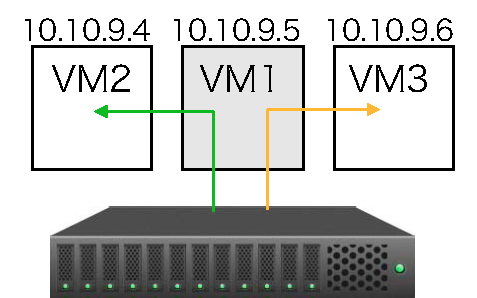
\includegraphics[width=65mm]{pics/env1.pdf}
	\caption{Direction of flows in experiment1}
	\label{fig: exp1}
\end{figure*}

\begin{figure*}
	\centering
	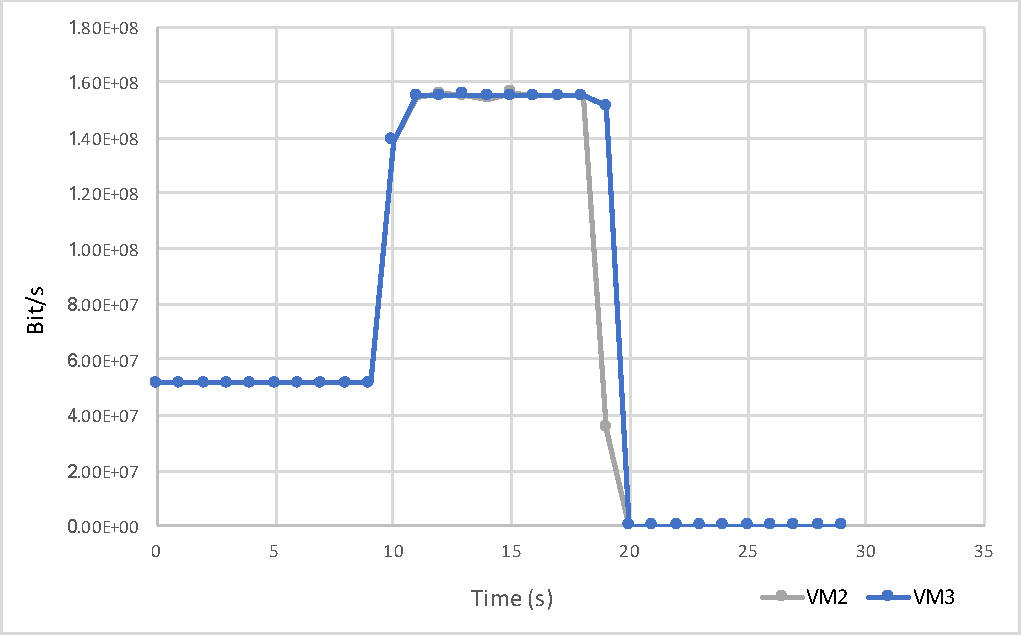
\includegraphics[width=120mm]{pics/throughput.pdf}
	\caption{Throughput at VM2 and VM3}
	\label{fig: result1}
\end{figure*}

\section{NF Chaining Performance}
To evaluate the performance of NF chaining, the following Experiment 1 is conducted. On VM1, Kernel-based NFCI executes chaining of two NFs, DoS Attack Denial (DAD) and DNAT. 

DAD counts the number of packets per flow. If in the previous 10 seconds the counter exceeds the threshold, all the packet in the flow will be dropped for the next 10 seconds. For this experiment the threshold of any flow is set to be 100Mbps. 

The chaining proceeds as follows: Hypervisor sends out two UDP flows to VM1 (10.10.9.5), flow1 having destination port number 53 (DNS protocol) and another flow2 having destination port number 123. The traffic is first chained with DAD and if the packet is not dropped, DNAT is processed. DNAT changes destination IP address to 10.10.9.4 (VM2) if it is flow1 and to 10.10.9.6 if it is flow2. So as shown in Fig. \ref{fig: exp1}, two flows originally destined to VM1 is split to VM2 and VM3. 

These two flows are sent for 30 seconds, first 10 seconds at rate of 50Mbps, next 10 seconds at 150Mbps and last 10 seconds at 100Mbps. 

The throughputs at VM2 and VM3 are shown in Figure \ref{fig: result1}.
Since both of the throughputs have similar value, it proves that the DNAT is working properly to split two flows to VM2 and VM3. The last 10 seconds both of flows have 0Mbps throughput. This is because from 10 to 20 seconds the traffic is exceeding 100Mbps and DAD starts dropping all the packet from 20s. 


\section{Evaluation of Resource Consumption}
Resource consumption when NF chaining is running to process traffic of 1Gbps $\times 2 $ is evaluated. Similar to Experiment 1, two UDP flows are sent to VM1 and split to VM2 and VM3 by DNAT. The difference is that the the two flow is transmitted at rate of 1Gbps for only 10 seconds. So the first NF DAD will work only as packet counting and blocking of packets will not triggered because there will be not packets in the next 10 seconds. Values of memory usage and CPU utilization are measured by vmstat command. 

When idle (no traffic processing is running), average memory usage was 766,664 Kbytes. When NF chaining at rate of 1Gbps $\times 2 $ is taking place, there were only average 20Kbytes of increase. CPU utilization showed nearly 0\% in both case of idle and processing. This indicates that NF chaining requires little amount of CPU processing. To get detailed information about used CPU time, I used dynamic tracing tool "BCC". Especially, a program that summarizes task on-CPU time as histogram is used. This shows how long tasks spent on the CPU before being descheduled. As shown in \ref{fig: cpudist}, the number of tasks that are on-CPU for 2048-4095 usecs is the highest in both cases when processing and idle. And the number of tasks when processing is roughly twice as high as when idle. CPU utilization is calculated using \ref{fig: cpudist} as following: To divide integral value of $time*10^-6 * number \: of \: tasks \: on \: time$ by $10*4$. And according to this calculation, CPU utilization is 0.059\% when processing and 0.034\% when idle. In summary, it costs about twice the CPU time for processing but the overall CPU utilization still remains nearly 0\%. 

\begin{table}
	\centering
	\begin{tabular}{|c|c|c|}
	\hline
	 & idle & processing \\
	 \hline
	 Memory Usage (KByte) & 766664 & 766844 \\
	 \hline
	 CPU Utilization (\%) & 0 & 0 \\
	 \hline
	\end{tabular}
	\caption{Comparison of resource consumption}
	\label{tbl: resource}
\end{table}

\begin{figure*}
	\centering
	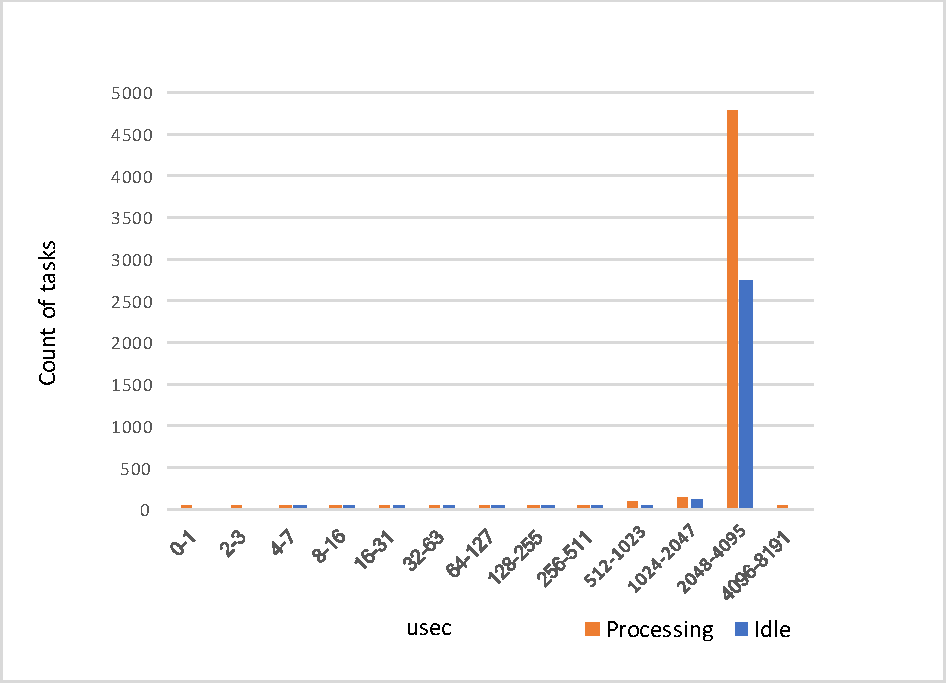
\includegraphics[width=120mm]{pics/cpudist.pdf}
	\caption{Histogram of tasks on-CPU time}
	\label{fig: cpudist}
\end{figure*}

\section{Evaluation of NF chaining at high traffic rate}
In addition to the evaluation of resource consumption in Experiment 2, throughput is measured here. As comparison, the throughput when routing the same flows on generic OS is measured, as shown in Fig. \ref{fig: env2}. Table \ref{tbl: throughput} shows that throughputs of both flows in NFC have only few kilobytes less than just routing. This proves that NFC provides equally well throughput compared with only routing at 1Gbps.

\begin{figure*}
	\centering
	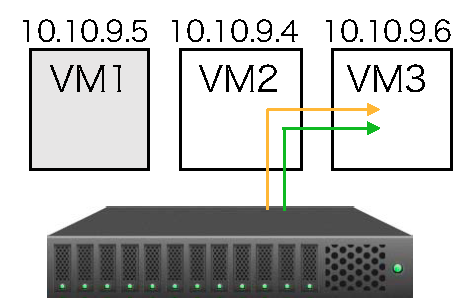
\includegraphics[width=65mm]{pics/env2.pdf}
	\caption{Routing of flows among general OSs}
	\label{fig: env2}
\end{figure*}

\begin{table}
	\centering
	\begin{tabular}{|c|c|c|}
	\hline
	 & Routing & NFC \\
	 \hline
	 flow1 (Kbps) & 801.6 & 797 \\
	 \hline
	 flow2 (Kbsp) & 804 & 800 \\
	 \hline
	\end{tabular}
	\caption{Comparison of throughput}
	\label{tbl: throughput}
\end{table}








\chapter{結論}
\label{chap:conclusion}
\section{Summary}
NFV brought innovation in telecommunication network by virtualizing NF and therefore adding flexibility in NF deployment. However, virtualization involves overhead in terms of memory copy and resource consumption. In order to eliminate these overhead as much as possible, I proposed lightweight NF chaining mechanism in kernel. The main idea of this proposal is that only complicated NFs are placed in user space and other simple NFs should be chained inside kernel. 

Among proposed architecture, the NF chaining in the kernel space is implemented. NF consists of kernel module(s) and the functions in the modules are registered to make a NF chain. The rule that decides which flow to pass specific NF chain is implemented by Filter table in Netfilter. User on the host can make a new NF chain or insert a NF in preexisting chain. By specifying rule for the chain, desired flow will be processed by the NF chain. 

Two NFs, DoS Attack Denial (DAD) and DNAT, are implemented to test the chaining mechanism. DAD counts received packets per flow and trigger blocking of the traffic if the count exceeds a threshold. DNAT changes the destination address /destination port number and was coordinated with connection tracking system in the Netfitler to achieve stateful process. 

Basic performance is evaluated by chaining the above two NFs. When two flows at 1Gbps rate are processed by the NF chain, resource consumption is measured. Memory usage raised only by a few tens of kilobytes compared to when the host is idle. And the CPU utilization remained 0\% when processing. By this measurement, it was confirmed that our NF chaining can be realized with very lightly in terms of CPU and memory usage. 

\section{Future Work}
The proposed architecture at this point only supports per packet process. For NF like ALG that need to read the original application message, the mechanism to reassemble split packets is necessary. The mechanism could be structured as follows: Every time a packet arrives, a kernel thread is created. If the packet is not the last one to make the original message, the thread is suspended by condition variable and the packet is inserted in a buffer. When the last packet arrives, the process of NF finally starts by passing the reassembled packets from the buffer. After completing the process the kernel threads is restarted so the suspended packets are free to proceed. 

\chapter*{謝辞}
\addcontentsline{toc}{chapter}
{\protect\numberline {}謝辞}
Foremost, I would like to express my sincere gratitude to my advisor Prof. Fumio Teraoka for the continuous support of my bachelor thesis study and research. His guidance helped me all the time in research and writing of this thesis. 

Besides my advisor, I am deeply grateful to my mentor Assistant Prof. Takao Kondo. Without his help and contribution this thesis would not have been possible.

Finally, I would like to thank my family for providing me with unfailing support and continuous encouragement throughout my years of study and the process of researching and writing thesis. 

This accomplishment would not have been possible without them. Thank you. 

Hanna Yoshimochi




%%%%%    参考文献    %%%%%
\typeout{References}
%%------------
\thispagestyle{plain}
%\bibliographystyle{junsrt}
\bibliographystyle{IEEEtran}
\bibliography{b-thesis}
\end{document}
